
\documentclass[11pt, a4paper]{article}

\usepackage[T1]{fontenc}
\usepackage{mathpazo}
\usepackage{graphicx}\graphicspath{{Images/}}
\usepackage[margin=1in]{geometry}
\usepackage{setspace}
\usepackage{caption,subcaption}
\usepackage[sort&compress, numbers]{natbib}
\usepackage{hyperref}

\captionsetup{font={small, stretch=1}, labelfont=bf}
\renewcommand{\figurename}{Fig.}
\setlength{\bibsep}{3pt}
\newcommand{\Title}[1]{{\LARGE \centering \hrulefill\\ \textbf{#1}\\ \hrulefill}}
%==================================================================

\begin{document}

\pagenumbering{roman}
\pagestyle{plain}


\onehalfspacing
\setcounter{page}{1}
\pagenumbering{arabic}
\Title{Computational Experience with the Maximal Location Covering Problem}

\section*{Abstract}
{\small \singlespacing
	On this paper, you can find heuristic approaches applied to the Maximal Covering Location Problems; this project could be useful to decision makers that want to generate a solution and try to improve a given solution as well in a short amount of time.  
}

\section{Introduction}\label{sec:intro}
Facility Location is a branch of Operations Research. This category of combinatorial optimization problems often deals with problems that seek to select the placement of a facility (often, from a given list of possibilities) that meets the best of certain constraints. These problems often consists of minimizing the total weighted distances from supplies and customers, and weights are representative of the difficulty of transporting materials. 

Then, we have the Maximal Covering Location Problem. This problem is a derivative of Facility Location sort; however, this problems seeks to maximize the customers covered by a given set of facilities,instead of minimizing the distance between customers and supplies. 

The Maximal Covering Location Problem (MCLP), is a classic problem in location analysis with    applications in a good number of fields, such as health care, emergency planning, ecology, statistical classification, homeland security, etc.

The objective of the MCLP is to maximize the population covered by a given set of facilities; however, this could work as an analogy to another problems that involve "supply" and "demand" points to maximize the demand as much as possible.

Formally, this problem is described in Church and ReVelle 1974 as follows:
"The maximal covering location problem seeks the maximum population which can be served within a stated service distance or time given a limited number of facilities."

In this work, MCLP is analysed and solved on random instances generated within a certain range, by an implemented instance generator. A Constructive Heuristic approach was used to generate a solution, and a Local Search algorithm was implemented to try to improve the feasible solution generated by the constructive. Overall, the effectiveness and computational time of the implemented algorithms on small, medium and large instances were analysed. More details are given in the following sections.

\section{Problem description - Mathematical model}\label{sec:lit}
According to the model defined on Church and ReVelle 1974, this problem is defined on a network of nodes and arcs. 

A mathematical formulation of this problem can be stated as Eq. ~\ref{eq: math model}:

\begin{equation}\label{eq: math model}
	max \; z = \sum_{i \in I}y_i
\end{equation}
subject to:

\begin{equation}\label{eq: r1}
	x_{j} \in (0,1), j \in J
\end{equation}

\begin{equation}\label{eq: r2}
	y_{i} \in (0,1), i \in I
\end{equation}

\begin{equation}\label{eq: r3}
	\sum_{j \in J}x_j = S
\end{equation}

\begin{equation}\label{eq: r4}
	\sum_{j \in N_i} x_j \geq y_i, N_i = \big\{ j \in J: d_{ij} \leq r \big\}
\end{equation}
where

\begin{itemize}
	\item $x_{j}$ : denotes that the $j$-th facility site is selected (1) or not (0). Boolean variable.
	\item $y_{i}$ : denotes that if the demand point i is covered by any facility site within radius $r$ (1) or not (0). Boolean variable.
	\item $I$ : the set of demand or population points. Array of indexes referencing the coordinates of each demand point.
	\item $J$ : the set of facility candidate sites. Array of indexes referencing the supply points.
	\item $d(i,j)$ : the Euclidean distance from a demand point $i$ to facility site $j$. 2-D matrix.
	\item $S$ : the number of desired facilities to be selected from the candidate sites $J$. Integer variable.
	\item $r$ : Maximal distance where a demand point from set $I$ is covered by a facility site from set $J$. Integer variable.
\end{itemize}
The objective is to maximize the number of demand points covered within a desired service distance, as depicted in ~\ref{eq: math model}.
A selection criteria for a site is described in restriction ~\ref{eq: r1}, where as restriction ~\ref{eq: r2} alludes to all the demands point covered within a specified radius. Ideally, the sum of the selected sites must be equal to the desired by a decision maker as stated on restriction ~\ref{eq: r3}; however, it's possible that all the demand/population points are covered before this restriction is satisfied. Restriction ~\ref{eq: r4} indicates that the distance between covered nodes by the selected sites must be under the specified radius from the user.

\subsection{Example}
The scatter plot shown in the figure ~\ref{fig:example_instance_input} was generated by an instance generator coded in the programming language Python. The range of the population points are within a range of 5-500 units, and the potential candidate sites were generated inside the convex hull of the demand points. There are exactly 500 demand points, and 20 candidate sites. The values were generated randomly.

\begin{figure}[h]
	\centering
	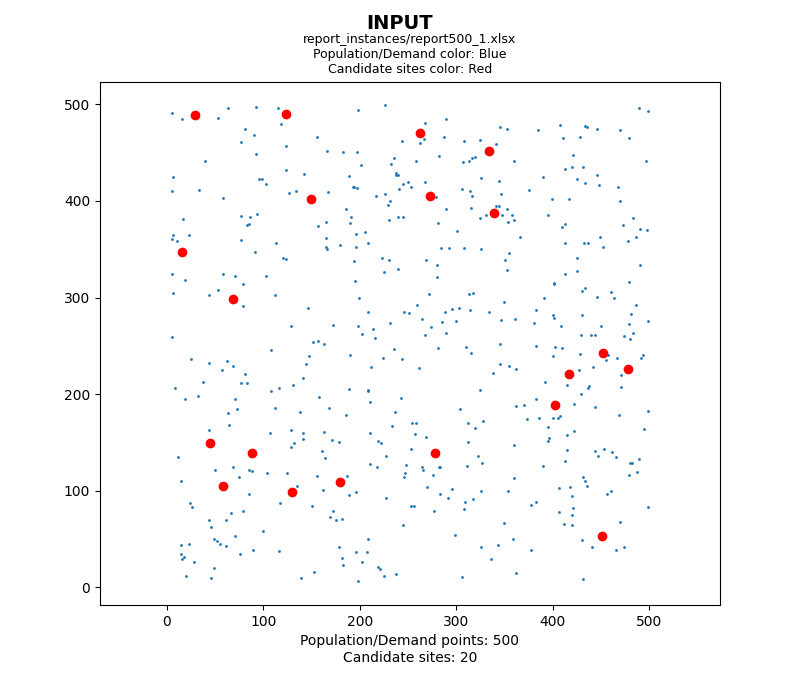
\includegraphics[scale=0.8]{example_instance_input.png}
	\caption{Random instance of population and candidate sites points}
	\label{fig:example_instance_input}
\end{figure}

As shown, the population points are illustrated in the scatter plot in blue, and the potential candidate sites are filled with red.

Once the input is succesfully computed, there are a few ways to figure out a first feasible solution. As seen in Church and ReVelle 1974, a first heuristic approach called Greedy Adding (GA) was considered. This approach starts with an empty solution, and starts to iterate each candidate site until the one with maximal covered population is found; then, this site is added to the solution. It keeps iterating until either the $S$ facilities have been selected or all the population is covered. However, there is a problem with this approach: the time complexity is denoted as $O(n \ logn)$, which means that it's not efficient for big instances.

Instead of using the Greedy Adding algorithm proposed by these guys, a Constructive Heuristic approach was implemented for generating first a feasible solution that meet the constraints. Then, a Local Search move approach tries to improve this solution. These heuristics are discused in more detail on the following sections.

\begin{figure}[h]
	\centering
	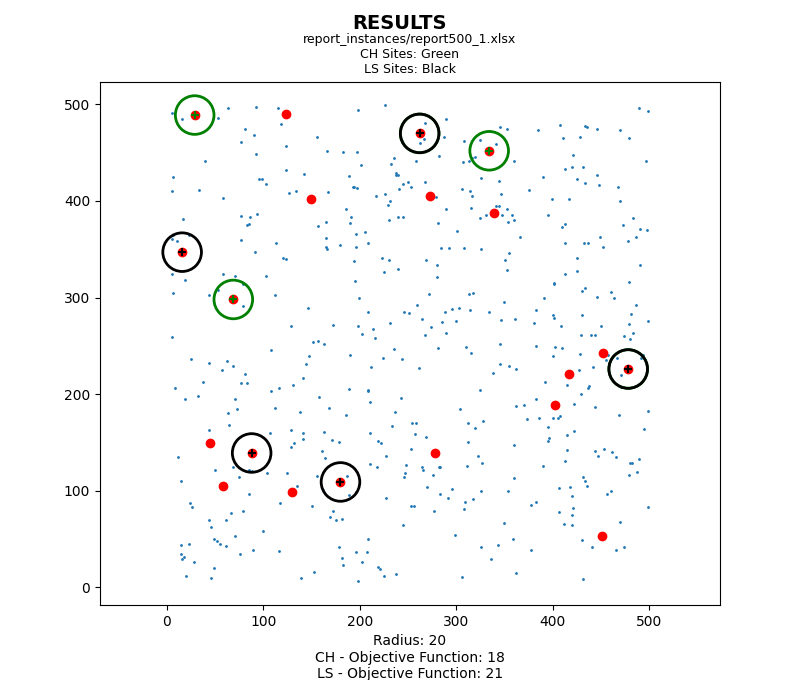
\includegraphics[scale=0.8]{example_instance_output.png}
	\caption{Random instance of population and candidate sites points}
	\label{fig:example_instance_output}
\end{figure}

The scatter plot shown in the figure ~\ref{fig:example_instance_output} illustrates the output of the applied heuristics mentioned previously. The sites and population covered of the Constructive Heuristic approach are marked with green circles, and black circles illustrate the ones covered by Local Search. 

\section{Heuristics}\label{sec:exp}

\subsection{Description of Constructive Heuristic}
An experiment is a procedure carried out to support, refute, or validate a hypothesis. Experiments provide insight into cause-and-effect by demonstrating what outcome occurs when a particular factor is manipulated. Experiments vary greatly in goal and scale, but always rely on repeatable procedure and logical analysis of the results. There also exists natural experimental studies.

A child may carry out basic experiments to understand gravity, while teams of scientists may take years of systematic investigation to advance their understanding of a phenomenon. Experiments and other types of hands-on activities are very important to student learning in the science classroom. Experiments can raise test scores and help a student become more engaged and interested in the material they are learning, especially when used over time. Experiments can vary from personal and informal natural comparisons (e.g. tasting a range of chocolates to find a favorite), to highly controlled (e.g. tests requiring complex apparatus overseen by many scientists that hope to discover information about subatomic particles). Uses of experiments vary considerably between the natural and human sciences. Fig.~\ref{fig:parabolic} is the parabolic plot.


\subsubsection{First subsubsection}
An experiment usually tests a hypothesis, which is an expectation about how a particular process or phenomenon works. However, an experiment may also aim to answer a ``what-if'' question, without a specific expectation about what the experiment reveals, or to confirm prior results. If an experiment is carefully conducted, the results usually either support or disprove the hypothesis. According to some philosophies of science, an experiment can never "prove" a hypothesis, it can only add support. On the other hand, an experiment that provides a counterexample can disprove a theory or hypothesis, but a theory can always be salvaged by appropriate ad hoc modifications at the expense of simplicity. An experiment must also control the possible confounding factors—any factors that would mar the accuracy or repeatability of the experiment or the ability to interpret the results. Confounding is commonly eliminated through scientific controls and/or, in randomized experiments, through random assignment.

In engineering and the physical sciences, experiments are a primary component of the scientific method. They are used to test theories and hypotheses about how physical processes work under particular conditions (e.g., whether a particular engineering process can produce a desired chemical compound). Typically, experiments in these fields focus on replication of identical procedures in hopes of producing identical results in each replication. Random assignment is uncommon.

\paragraph{Paragraph tile.}
According to his explanation, a strictly controlled test execution with a sensibility for the subjectivity and susceptibility of outcomes due to the nature of man is necessary.

\subsection{Description of Local Search}
In engineering and the physical sciences, experiments are a primary component of the scientific method. They are used to test theories and hypotheses about how physical processes work under particular conditions (e.g., whether a particular engineering process can produce a desired chemical compound). Typically, experiments in these fields focus on replication of identical procedures in hopes of producing identical results in each replication. Random assignment is uncommon.

\section{Experiments}\label{sec:conc} 
Conclusions show readers the value of your completely developed argument or thoroughly answered question. Consider the conclusion from the reader's perspective. At the end of a paper, a reader wants to know how to benefit from the work you accomplished in your paper. 

\section{Conclusions}
Conclusions show readers the value of your completely developed argument or thoroughly answered question. Consider the conclusion from the reader's perspective. At the end of a paper, a reader wants to know how to benefit from the work you accomplished in your paper. 

\appendix
\section{Supporting information}
The purpose of the supporting information is to enable authors to provide and archive supporting information such as data tables, method information, figures, video, or computer software, in digital formats so that other scientists can use it.

\small \singlespacing
\bibliographystyle{unsrtnat} 
\bibliography{mybib}

\end{document}









 





















